%%
%% Automatically generated file from DocOnce source
%% (https://github.com/hplgit/doconce/)
%%

% #define PREAMBLE

% #ifdef PREAMBLE
%-------------------- begin preamble ----------------------

\documentclass[%
oneside,                 % oneside: electronic viewing, twoside: printing
final,                   % draft: marks overfull hboxes, figures with paths
10pt,french]{article}

\listfiles               %  print all files needed to compile this document

\usepackage{relsize,makeidx,color,setspace,amsmath,amsfonts,amssymb}
\usepackage[table]{xcolor}
\usepackage{bm,ltablex,microtype}

\usepackage[pdftex]{graphicx}

% Packages for typesetting blocks of computer code
\usepackage{fancyvrb,framed,moreverb}

% Define colors
\definecolor{orange}{cmyk}{0,0.4,0.8,0.2}
\definecolor{tucorange}{rgb}{1.0,0.64,0}
\definecolor{darkorange}{rgb}{.71,0.21,0.01}
\definecolor{darkgreen}{rgb}{.12,.54,.11}
\definecolor{myteal}{rgb}{.26, .44, .56}
\definecolor{gray}{gray}{0.45}
\definecolor{mediumgray}{gray}{.8}
\definecolor{lightgray}{gray}{.95}
\definecolor{brown}{rgb}{0.54,0.27,0.07}
\definecolor{purple}{rgb}{0.5,0.0,0.5}
\definecolor{darkgray}{gray}{0.25}
\definecolor{darkblue}{rgb}{0,0.08,0.45}
\definecolor{darkblue2}{rgb}{0,0,0.8}
\definecolor{lightred}{rgb}{1.0,0.39,0.28}
\definecolor{lightgreen}{rgb}{0.48,0.99,0.0}
\definecolor{lightblue}{rgb}{0.53,0.81,0.92}
\definecolor{lightblue2}{rgb}{0.3,0.3,1.0}
\definecolor{lightpurple}{rgb}{0.87,0.63,0.87}
\definecolor{lightcyan}{rgb}{0.5,1.0,0.83}

\colorlet{comment_green}{green!50!black}
\colorlet{string_red}{red!60!black}
\colorlet{keyword_pink}{magenta!70!black}
\colorlet{indendifier_green}{green!70!white}

% Backgrounds for code
\definecolor{cbg_gray}{rgb}{.95, .95, .95}
\definecolor{bar_gray}{rgb}{.92, .92, .92}

\definecolor{cbg_yellowgray}{rgb}{.95, .95, .85}
\definecolor{bar_yellowgray}{rgb}{.95, .95, .65}

\colorlet{cbg_yellow2}{yellow!10}
\colorlet{bar_yellow2}{yellow!20}

\definecolor{cbg_yellow1}{rgb}{.98, .98, 0.8}
\definecolor{bar_yellow1}{rgb}{.98, .98, 0.4}

\definecolor{cbg_red1}{rgb}{1, 0.85, 0.85}
\definecolor{bar_red1}{rgb}{1, 0.75, 0.85}

\definecolor{cbg_blue1}{rgb}{0.87843, 0.95686, 1.0}
\definecolor{bar_blue1}{rgb}{0.7,     0.95686, 1}

%\setlength{\fboxsep}{-1.5mm}  % adjust cod_vpad/pro_vpad background box

%% Background for code blocks (parameter is color name)

%% pro/cod_vpad: gives some vertical padding before and after the text
%% (but has more simplistic code than _cod/pro_tight+cod/pro).
%% pro/cod_vpad can be used to enclose Verbatim or lst begin/end for code.
%% pro/cod calls _pro/cod_tight and has very little vertical padding,
%% used to enclose Verbatim and other begin/end for code.
%% (pro/cod is what the ptex2tex program could produce with the
%% Blue/BlueBar definitions in .ptex2tex.cfg.)

\newenvironment{cod_vpad}[1]{
   \def\FrameCommand{\colorbox{#1}}
   \MakeFramed{\FrameRestore}}
   {\endMakeFramed}

\newenvironment{_cod_tight}[1]{
   \def\FrameCommand{\colorbox{#1}}
   \FrameRule0.6pt\MakeFramed {\FrameRestore}\vskip3mm}
   {\vskip0mm\endMakeFramed}

\newenvironment{cod}[1]{
\bgroup\rmfamily
\fboxsep=0mm\relax
\begin{_cod_tight}{#1}
\list{}{\parsep=-2mm\parskip=0mm\topsep=0pt\leftmargin=2mm
\rightmargin=2\leftmargin\leftmargin=4pt\relax}
\item\relax}
{\endlist\end{_cod_tight}\egroup}

%% Background for complete program blocks (parameter 1 is color name
%% for background, parameter 2 is color for left bar)
\newenvironment{pro_vpad}[2]{
   \def\FrameCommand{\color{#2}\vrule width 1mm\normalcolor\colorbox{#1}}
   \MakeFramed{\FrameRestore}}
   {\endMakeFramed}

\newenvironment{_pro_tight}[2]{
   \def\FrameCommand{\color{#2}\vrule width 1mm\normalcolor\colorbox{#1}}
   \FrameRule0.6pt\MakeFramed {\advance\hsize-2mm\FrameRestore}\vskip3mm}
   {\vskip0mm\endMakeFramed}

\newenvironment{pro}[2]{
\bgroup\rmfamily
\fboxsep=0mm\relax
\begin{_pro_tight}{#1}{#2}
\list{}{\parsep=-2mm\parskip=0mm\topsep=0pt\leftmargin=2mm
\rightmargin=2\leftmargin\leftmargin=4pt\relax}
\item\relax}
{\endlist\end{_pro_tight}\egroup}

\usepackage{minted}
\usemintedstyle{default}

\usepackage[T1]{fontenc}
%\usepackage[latin1]{inputenc}
\usepackage{ucs}
\usepackage[utf8x]{inputenc}

\usepackage{lmodern}         % Latin Modern fonts derived from Computer Modern

% Hyperlinks in PDF:
\definecolor{linkcolor}{rgb}{0,0,0.4}
\usepackage{hyperref}
\hypersetup{
    breaklinks=true,
    colorlinks=true,
    linkcolor=linkcolor,
    urlcolor=linkcolor,
    citecolor=black,
    filecolor=black,
    %filecolor=blue,
    pdfmenubar=true,
    pdftoolbar=true,
    bookmarksdepth=3   % Uncomment (and tweak) for PDF bookmarks with more levels than the TOC
    }
%\hyperbaseurl{}   % hyperlinks are relative to this root

\setcounter{tocdepth}{2}  % levels in table of contents

% Tricks for having figures close to where they are defined:
% 1. define less restrictive rules for where to put figures
\setcounter{topnumber}{2}
\setcounter{bottomnumber}{2}
\setcounter{totalnumber}{4}
\renewcommand{\topfraction}{0.95}
\renewcommand{\bottomfraction}{0.95}
\renewcommand{\textfraction}{0}
\renewcommand{\floatpagefraction}{0.75}
% floatpagefraction must always be less than topfraction!
% 2. ensure all figures are flushed before next section
\usepackage[section]{placeins}
% 3. enable begin{figure}[H] (often leads to ugly pagebreaks)
%\usepackage{float}\restylefloat{figure}

% --- fancyhdr package for fancy headers ---
\usepackage{fancyhdr}
\fancyhf{} % sets both header and footer to nothing
\renewcommand{\headrulewidth}{0pt}
\fancyfoot[LE,RO]{\thepage}
% Ensure copyright on titlepage (article style) and chapter pages (book style)
\fancypagestyle{plain}{
  \fancyhf{}
  \fancyfoot[C]{{\footnotesize \copyright\ 2020, Ahmed Ammar. Released under CC Attribution 4.0 license}}
%  \renewcommand{\footrulewidth}{0mm}
  \renewcommand{\headrulewidth}{0mm}
}
% Ensure copyright on titlepages with \thispagestyle{empty}
\fancypagestyle{empty}{
  \fancyhf{}
  \fancyfoot[C]{{\footnotesize \copyright\ 2020, Ahmed Ammar. Released under CC Attribution 4.0 license}}
  \renewcommand{\footrulewidth}{0mm}
  \renewcommand{\headrulewidth}{0mm}
}

\pagestyle{fancy}


% prevent orhpans and widows
\clubpenalty = 10000
\widowpenalty = 10000

\newenvironment{doconceexercise}{}{}
\newcounter{doconceexercisecounter}
% --- begin definition of \listofexercises command ---
\makeatletter
\newcommand\listofexercises{\section*{List of Exercices}
\@starttoc{loe}
}
\newcommand*{\l@doconceexercise}{\@dottedtocline{0}{0pt}{6.5em}}
\makeatother
% --- end definition of \listofexercises command ---



% ------ header in subexercises ------
%\newcommand{\subex}[1]{\paragraph{#1}}
%\newcommand{\subex}[1]{\par\vspace{1.7mm}\noindent{\bf #1}\ \ }
\makeatletter
% 1.5ex is the spacing above the header, 0.5em the spacing after subex title
\newcommand\subex{\@startsection{paragraph}{4}{\z@}%
                  {1.5ex\@plus1ex \@minus.2ex}%
                  {-0.5em}%
                  {\normalfont\normalsize\bfseries}}
\makeatother


% --- end of standard preamble for documents ---


% insert custom LaTeX commands...

\raggedbottom
\makeindex
\usepackage[totoc]{idxlayout}   % for index in the toc
\usepackage[nottoc]{tocbibind}  % for references/bibliography in the toc

%-------------------- end preamble ----------------------

\begin{document}

% matching end for #ifdef PREAMBLE
% #endif

\newcommand{\exercisesection}[1]{\subsection*{#1}}


% ------------------- main content ----------------------



% ----------------- title -------------------------

\thispagestyle{empty}

\begin{center}
{\LARGE\bf
\begin{spacing}{1.25}
TD N°6 : Résolution des équations aux dérivées partielles
\end{spacing}
}
\end{center}

% ----------------- author(s) -------------------------

\begin{center}
{\bf Ahmed Ammar (\texttt{ahmed.ammar@fst.utm.tn})}
\end{center}

    \begin{center}
% List of all institutions:
\centerline{{\small Institut Préparatoire aux Études Scientifiques et Techniques, Université de Carthage.}}
\end{center}
    
% ----------------- end author(s) -------------------------

% --- begin date ---
\begin{center}
Apr 22, 2020
\end{center}
% --- end date ---

\vspace{1cm}


\tableofcontents


\vspace{1cm} % after toc



% !split


% --- begin exercise ---
\begin{doconceexercise}
\refstepcounter{doconceexercisecounter}

\exercisesection{Exercice \thedoconceexercisecounter: Équation de la chaleur 2D}


On considère une plaque de fer carrée de côté L = 10 mm, de coefficient de diffusion D = 4 $mm^2.s^{-1}$.

L'équation de diffusion bidimensionnelle est
\begin{equation}
\frac{\partial U}{\partial t} = D\left(\frac{\partial^2U}{\partial x^2} + \frac{\partial^2U}{\partial y^2} \right)
\end{equation}
Considérons l'équation de diffusion appliquée à une plaque métallique carrée de côté L = 10 mm, de coefficient de diffusion D = 4 $mm^2.s^{-1}$. La plaque est initialement à la température $T_{froid} = 300 \ K$ en dehors d'un disque (centré sur $x_c$ = 5, $y_c$ =5 et de rayon r = 2 mm) qui est à la température $T_{chaud} = 1000 \ K$. Nous supposons que les bords de la plaque sont maintenus fixes à $T_{froid}$.


\subex{a)}
Rappeler la définition d'un schéma FTCS et donner l’approximation numérique de l'équation de chaleur 2D.


% --- begin solution of exercise ---
\paragraph{Solution.}
Le schéma FTCS (Forward Time Centred Space) est un schéma explicite d'ordre 1 en temps et d'ordre 2 en espace. Il s'agit de discrétiser les deux dérivées partielles en utilisant un développement de Taylor. Le membre de gauche peut donc s'écrire en approximant :
\begin{equation}
u_{i,j}^{(n+1)} = u_{i,j}^{(n)} + D\Delta t\left[ \frac{u_{i+1,j}^{(n)} - 2u_{i,j}^{(n)} + u_{i-1,j}^{(n)}}{(\Delta x)^2} + \frac{u_{i,j+1}^{(n)} - 2u_{i,j}^{(n)} + u_{i,j-1}^{(n)}}{(\Delta y)^2} \right].
\end{equation}

% --- end solution of exercise ---

\subex{b)}
Quelle est la valeur du temps maximum $\Delta t$ que nous pouvons autoriser sans que le processus ne devienne instable?


% --- begin solution of exercise ---
\paragraph{Solution.}
On peut montrer que le pas de temps maximum, $\Delta t$ que nous pouvons autoriser sans que le processus ne devienne instable est :
\begin{equation}
\Delta t = \frac{1}{2D}\frac{(\Delta x\Delta y)^2}{(\Delta x)^2 + (\Delta y)^2}.
\end{equation}

% --- end solution of exercise ---

\subex{c)}
Terminer lorsqu'il y a des points d'interrogation ($???$) dans le script Python \texttt{EquDiff2D.py} ci-dessous afin d'obtenir la sortie comme indiqué dans la figure~\ref{fig:EquDiff2D}.
\begin{pro}{cbg_gray}{bar_gray}\begin{minted}[fontsize=\fontsize{9pt}{9pt},linenos=false,mathescape,baselinestretch=1.0,fontfamily=tt,xleftmargin=2mm]{python}
## NOM DU PROGRAMME: EquDiff2D.py
#% IMPORTATION
import numpy as np
import matplotlib.pyplot as plt
# taille de la plaque, en [mm]
L = 10.
# intervalles dans les directions x, y, en [mm]
dx = dy = 0.1
# Coefficient de diffusion thermique de l'acier, en [mm2.s-1]
D = 4.
Tfroid, Tchaud = 300, 1000
# Nombre de pas de temps
nsteps = 250
nx, ny = int(L/dx), int(L/dy)
dx2, dy2 = dx*dx, dy*dy
# pas de temps maximum, dans question b)
dt = ???
u = Tfroid * np.ones((nx, ny))
# Conditions initiales - disque de rayon r, centrée sur (cx, cy), en [mm]
r, cx, cy = 2, 5, 5
r2 = r**2
for i in range(nx):
    for j in range(ny):
        p2 = ???
        if p2 < r2:
            u[i,j] = Tchaud
# Sortie de 4 graphiques à quatre instants dans l'intervalle de temps
mfig = [0, 50, 100, 200]
fignum = 0 # initialisation
fig = plt.figure()
# implémentation du schéma FTCS
for m in range(nsteps):
    for i in range(1, nx-1):
        for j in range(1, ny-1):
            uxx = ???
            uyy = ???
            u[i,j] += ???
    if m in mfig:
        fignum += 1
        print(m, fignum)
        ax = fig.add_subplot(220 + fignum)
        im = ax.imshow(u, cmap=plt.get_cmap('hot'), vmin=Tfroid,vmax=Tchaud)
        ax.set_axis_off()
        ax.set_title('{:.1f} ms'.format(m*dt*1000))
fig.subplots_adjust(right=0.85)
cbar_ax = fig.add_axes([0.9, 0.15, 0.03, 0.7])
cbar_ax.set_xlabel('T [K]', labelpad=20)
fig.colorbar(im, cax=cbar_ax)
plt.savefig("EquDiff2D.png"); plt.savefig("EquDiff2D.pdf")
plt.show()
\end{minted}
\end{pro}
\noindent


\begin{figure}[!ht]  % fig:EquDiff2D
  \centerline{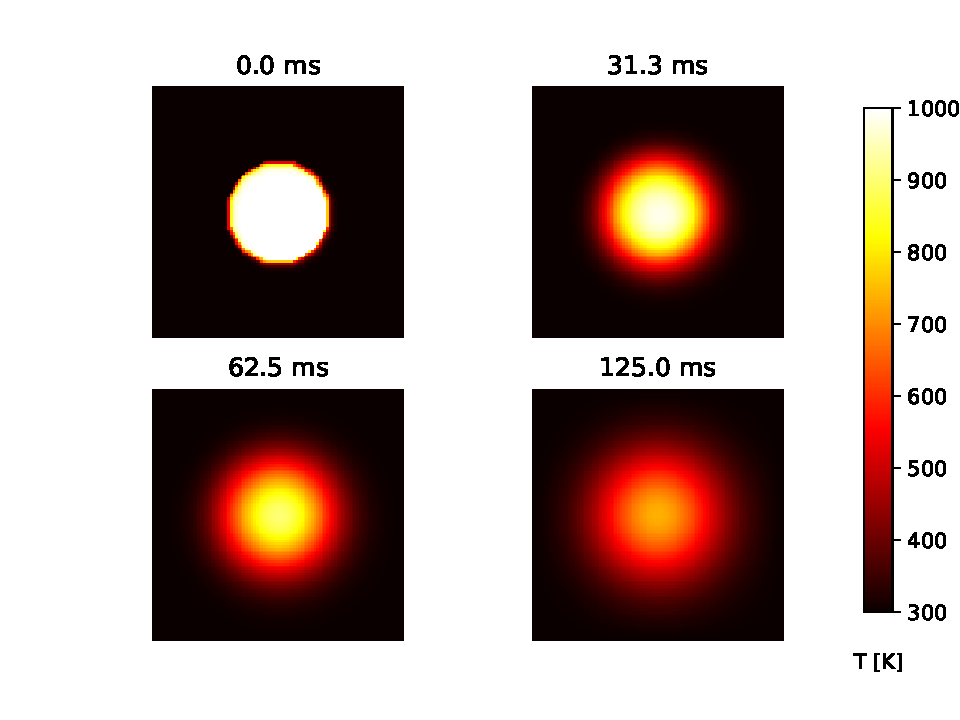
\includegraphics[width=0.8\linewidth]{scripts/EquDiff2D.pdf}}
  \caption{
  \label{fig:EquDiff2D}
  }
\end{figure}
%\clearpage % flush figures fig:EquDiff2D

% !split
% ===== Exercice:  Une équation d’onde en deux dimensions =====
% Modifiez l’exemple d’intégration en temps explicite de l’équation de la chaleur en deux dimensions (vu ci-dessus) pour traiter (toujours en deux dimensions) l’équation d’ondes suivante

\end{doconceexercise}
% --- end exercise ---


% !split


% --- begin exercise ---
\begin{doconceexercise}
\refstepcounter{doconceexercisecounter}

\exercisesection{Exercice \thedoconceexercisecounter: Condensateur plan}


Résoudre l'équation de Laplace en deux dimensions pour le potentiel dans un condensateur plan
\begin{align}
\dfrac{\partial^2 u(x, y)}{\partial x^2} + \dfrac{\partial^2 u(x, y)}{\partial y^2}  &= 0
\end{align}
Soit un condensateur à plaques parallèles avec des potentiels V = $\pm$ 1 V contenus dans une région carrée mise à la terre de longueur latérale L comme indiqué sur la figure~\ref{fig:laplace2DExercice}.


\begin{figure}[!ht]  % fig:laplace2DExercice
  \centerline{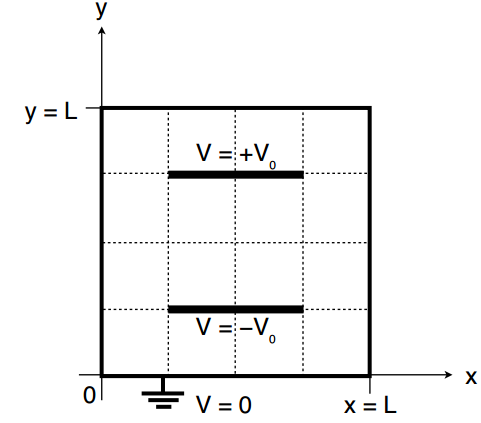
\includegraphics[width=0.5\linewidth]{imgs/laplace2DExercice.png}}
  \caption{
  \label{fig:laplace2DExercice}
  }
\end{figure}
%\clearpage % flush figures fig:laplace2DExercice



\subex{a)}
Rappeler la définition de la méthode Gauss-Seidel et donner l’approximation numérique de l'équation de Laplace 2D.

\subex{b)}
Adapter le script \Verb!Laplace_surrelax.py! étudié dans le cours afin d'avoir les résultats sur les figures~\ref{fig:Laplace_condensateur2D} et~\ref{fig:Laplace_condensateur3D}.


\begin{figure}[!ht]  % fig:Laplace_condensateur2D
  \centerline{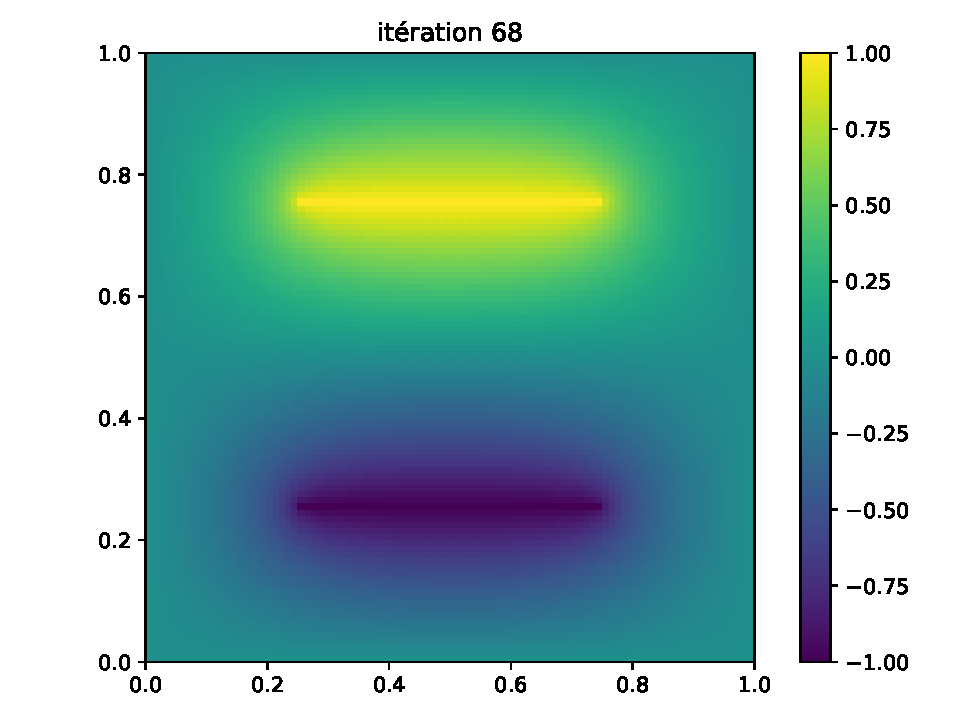
\includegraphics[width=1.0\linewidth]{scripts/Laplace_condensateur2D.pdf}}
  \caption{
  \label{fig:Laplace_condensateur2D}
  }
\end{figure}
%\clearpage % flush figures fig:Laplace_condensateur2D



\begin{figure}[!ht]  % fig:Laplace_condensateur3D
  \centerline{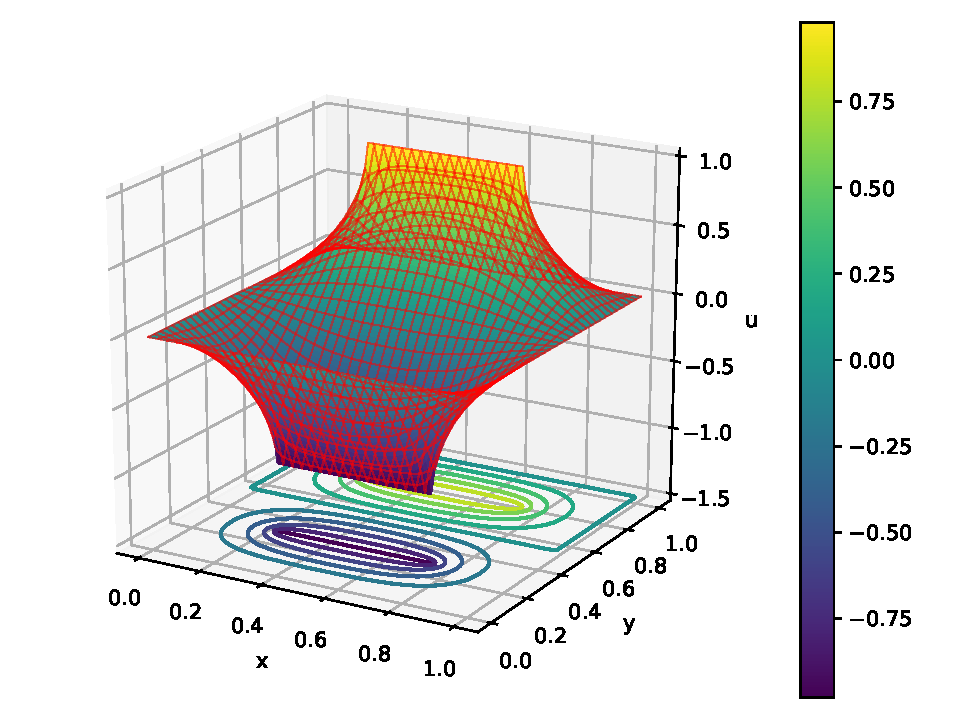
\includegraphics[width=1.0\linewidth]{scripts/Laplace_condensateur3D.pdf}}
  \caption{
  \label{fig:Laplace_condensateur3D}
  }
\end{figure}
%\clearpage % flush figures fig:Laplace_condensateur3D


\end{doconceexercise}
% --- end exercise ---


% ------------------- end of main content ---------------

% #ifdef PREAMBLE
\end{document}
% #endif

